\documentclass{article}


\usepackage[urlcolor=blue, linkcolor=black, colorlinks=true]{hyperref}
\usepackage[dutch]{babel}
\usepackage{minutes}
\usepackage{graphicx}

\renewcommand{\familydefault}{\sfdefault}


\makeatletter
\addto\extrasdutch{%
\def\min@textTask{Taak}%
}
\makeatother%
\makeatletter
\def\blfootnote{\gdef\@thefnmark{}\@footnotetext}
\makeatother




\newcounter{team}

% TODO: Enter team number here:
\setcounter{team}{6}


\begin{document}
%	\tableofcontents

	\begin{Minutes}{Programming Project Databases \\ Intermediate Evaluation Team \arabic{team}}
		\minutesdate{19 april 2020}

		\maketitle

		\topic{Status}
		    \subtopic{Page templates}
		    Our website pages are written using Bulma and Jinja2, based on HTML. Everyone has made and tweaked at least one of the front end pages for our web application. Here is an overview of who did which page.

    		    \subsubtopic{Arno}
    		        \task*[DONE]{Login page}
    			    \task*[DONE]{Home page (Logged in)}
    			    \task*[DONE]{Request page}
    			    \task*[DONE]{Route search page}
    			    \task*[DONE]{Error 404: Page not found}
    			    \task*[DONE]{Error 405: Method not allowed}
    			    \task*[DONE]{Error 500: Bad Gateaway}
    			    \task*[DONE]{W.I.P. page}
    			    \task*[DONE]{Route edit page}
    			\subsubtopic{Sam}
    			    \task*[DONE]{Home page}
    			    \task*[DONE]{Settings page}
    			    \task*[DONE]{Requests overview page}
    			\subsubtopic{Sien}
    			    \task*[DONE]{About page}
    			    \task*[DONE]{Account page}
    			    \task*[DONE]{History page}
    			\subsubtopic{Tim}
    			    \task*[DONE]{Add Route page}

    	 \subtopic{Page additional features}
    	 Most of our pages have small javascript elements, here is an overview of who did which part. We've used Leaflet for the maps and Nominatim as geocoding service.

    			\subsubtopic{Arno}
    		        \task*[DONE]{Burger icon}
    		        On the mobile version of our site, the navigation bar collapses into a burger icon. Since Bulma didn't include any javascript code, this had to be added manually.
    		        \task*[DONE]{Spotify playlist}
    		        Added a Spotify playlist to the route page. This gives you an example of what the music durint the trip might be like.
    			\subsubtopic{Sam}
    			    \task*[DONE]{Autocomplete Music Preference}
    			\subsubtopic{Sien}
    			    \task*[DONE]{View notifications on hover}
    			    By hovering over the notification icon, you get a list of the notifications. These contain requests and the next route that is planned in the future (if there is one)
    			    \task*[DONE]{View future routes on home page}
    			    Last time we used a given input instead of getting the routes from the database. Now the homepage shows you your future routes, if you have any, with the different stops and potential passengers.
    			    \task*[DONE]{History page}
    			    There has been added a new page where you find a table of all your past routes.
    			\subsubtopic{Tim}
    			    \task*[DONE]{Map}
    			    Create an interactive map and display a location markers on it.
    			    \task*[ABANDONED]{Auto complete addresses}
    			    We first wanted to automatically complete the addres a person is entering, but realized soon that this isn't allowed by Nominatim and decided to abandon this feature.

    	  \subtopic{Backend Flask}
    	        We're using Flask with a bunch of it's extensions as Web Server.
    	        \subsubtopic{Arno}
    			    \task*[DONE]{Registration}
    			    Adding the forms from the registration HTML in flask, accessing their contents and adding a new user to the database (if all inputs are correct).
    			    \task*[DONE]{GUI Login}
    			    Added validation for credentials, added functions to access the current user and added a check to pages where a login is required, to redirect them to the login page and after logging in getting automatically redirected back to the page you came from.
    			    \task*[DONE]{GUI search routes}
    			    \task*[DONE]{API create routes}
    			    Creating routes using the API
    			    \task*[DONE]{API deleting routes, request and user}
    			    Given the option to delete these elements using the API.
    			    \task*[DONE]{API updating route}
    			    Given the ability to update specific fields of the route using the API.
    			    \task*[DONE]{API check login}
    			    When accessing a API page where the login is required, this function decorator checks the token provided and load the current user for the time of the request.
    			\subsubtopic{Sam}
    			    \task*[DONE]{Settings}
    			    Adding the forms from the settings HTML in flask, and use their contents to edit the user settings.
    			    \task*[DONE]{Passenger Requests}
    			    Added support for passenger requests in the API.
    			    \task*[DONE]{ER-Diagram (second version)}
    			    Creating a second version of the ER-Diagram.
    			\subsubtopic{Sien}
    			    \task*[DONE]{Search routes}
    			    Added support for search routes in the API.
    			    \task*[DONE]{Notifications count}
    			    Added functions to get the number of notifications for users.
    			\subsubtopic{Tim}
    			    \task*[DONE]{ER-Diagram (first version)}
    			    Creating an initial version of the ER-Diagram.
    			    \task*[DONE]{Tokens}
    			    Adding support for checking if the received token is valid or not
    			    \task*[DONE]{Routes}
    			    Routes are now supported and relied upon by the service, It consists of the address of the start location and end location, the date and who created the creator of the route is.
    			    \task*[DONE]{Geolocator}
    			    Did some basic research over which geolocator to use and how to implement them. We ended up choosing for Nominatim which is completely free but at the cost of only being allowed to send 1 request each second. So some changes had to be made to make sure loading times weren't causing too much problems.


    	\subtopic{Database design}
    	    We're using SQLAlchemy and Psycopg2 to handle requests to our Postgress database. More info about the design can be found in the ER-Diagram section.

    	\subtopic{Unit testing}
    	    We've used Flask-Testing to perform a few test scenario's for the API.
    	    \subsubtopic{Arno}
    	        \task*[DONE]{Basic authentication test}
    	        Made a test scenario for registration and logging in, so the other team members had an example of how to use the test environment.

    	\subtopic{Deployment}
    	    \subsubtopic{Arno}
    	        \task*[DONE]{Updating the server}
    	        Regularly pulling our new changes from GitHub to the server.
    	        \task*[DONE]{Setting up our site}
    	        Setting up the service and Nginx to use our application instead of the template web app.
    	   \subtopic{Sam}
    	        \task*[DONE]{Setting up the VM}
    	        Creating a VM instance on GCP and deploying the template webapp on it.

    	\subtopic{Teamwork}
    	During our planning last week, we've tried to distribute the work so everyone can do their work and preventing merge conflicts as much as possible. Something that helped a lot with achieving this was restructuring our project, so only things closely related to each other were in the same file. As recommended at the beginning of the semester, we've given everyone some specific pages to focus on, so they can experience every part of the web development. The weekly meetings were also useful to help people somewhere if needed. For exampling in our plan for week 6, Tim focused on the page to add routes, Sien on the user page, Sam on the Music settings page and Arno on the request pages. This is a way to let everyone work independent, while accomplishing a finished project as a team.

    	\topic{API}
    	The API that's currently implemented is the minimum required API (described \href{https://ppdb.docs.apiary.io/}{here} with some extra route to apply the CRUD principle. You can find the documentation about our API \href{https://placeholder.docs.apiary.io/}{here}.

    	\topic{ER-Diagram}
    	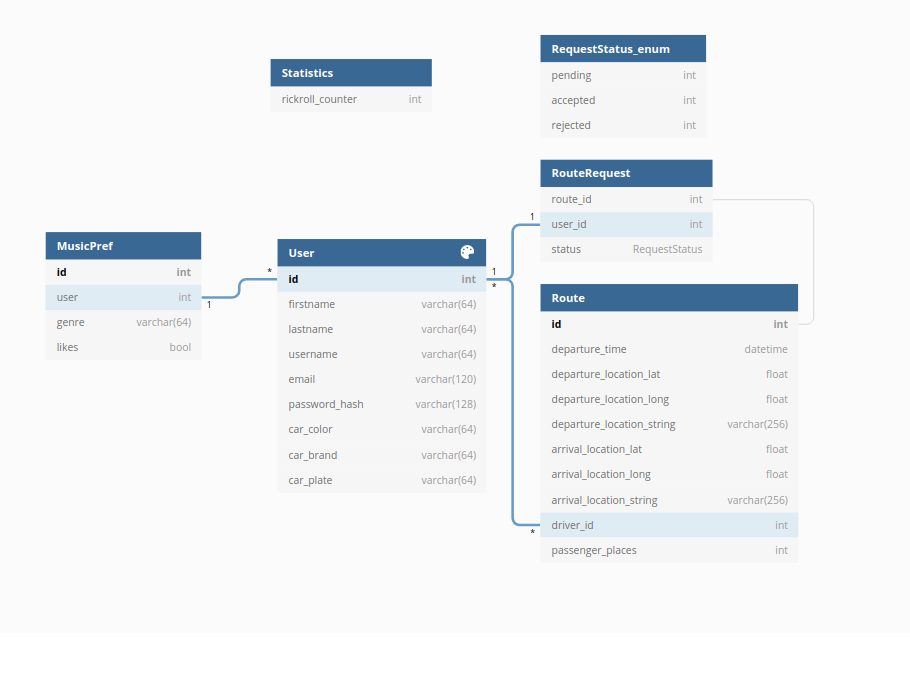
\includegraphics[scale=2]{ERD2.png}
    	    \subtopic{User}
            The user table has the standard fields:
            \begin{itemize}
                \item id (pk): Primary key, unique for each user
                \item firstname: The firstname of the user
                \item lastname: The lastname of the user
                \item username (unique): A unique username for loggin in
                \item email (unique): The email of the user
                \item password\_hash: A hashed version of the password
            \end{itemize}
            This table also keeps the info about the car of the user.
            These fields can be Null if the user doesn't have a car.
            \begin{itemize}
                \item car\_color
                \item car\_brand
                \item car\_plate
            \end{itemize}

            \subtopic{Route}
            The route table keeps the info about drives.
            \begin{itemize}
                \item departure\_time
                \item departure\_location\_lat
                \item departure\_location\_long
                \item departure\_location\_string
                \item arrival\_location\_lat
                \item arrival\_location\_long
                \item arrival\_location\_string
            \end{itemize}
            Location\_lat and long are the coordinates. location\_string is the string representation of the adres. We save this field in the db to minimise the amount of api requests to nomatim.
            \begin{itemize}
                \item driver\_id (fk: User.id)
                \item passenger\_places
            \end{itemize}

            A route can have one user as a driver. A user can be a driver for multiple routes. (User 1 to * Route)

            \subtopic{RequestStatus}
            An enum to represent the status of a passenger request.
            \begin{itemize}
                \item pending
                \item accepted
                \item rejected
            \end{itemize}

            \subtopic{RouteRequest}
            This table represents a passenger request. When a request is accepted, the user gets seen as a passenger. Passenger is not saved seperately in Route to prevent duplicates.
            \begin{itemize}
                \item route\_id (fk: Route.id)
                \item user\_id (fk: User.id)
                \item status
            \end{itemize}

            A request is for 1 route. A route can have multiple requests (Route 1 to * RouteRequest).
            The user\_id is for the user that made the request.
            A user can make multiple requests. A request can only be made by 1 user (User 1 to * RouteRequest).

            \subtopic{MusicPref}
            This table shows which genres a user (dis)likes.
            \begin{itemize}
                \item id (pk)
                \item user (fk: User.id)
                \item genre
                \item likes
            \end{itemize}

            A user can have multiple preferences. A preference points to 1 user (User 1 to * MusicPref).
            The likes field is true if the user likes the genre and false if disliked.
            This is stored in a seperate table (not in User) to get a better overview and prevent the User model gets too big.

        \topic{User journey}
        An example of how the user interacts with our website.
        When going to \href{team6.ppdb.me}, you can immediately go to the registration page by clicking on the primary Sign up button in the navigation bar. Here you can fill in the form. Once you've submitted your data, you get redirected to the login page, where you can sign in using the credentials you just entered. After signing in, you can see the main logged in page without any trips. Start by completing you settings, by clicking on "Settings" in the navigation bar. Here you can add information about your car, your music preferences, your email, ... Now click on "Home" in the navigation bar and add a route by entering them using Add a new trip. You can add a new trip from and to wherever you'd like on any date in the future, lets assume this user wants to add a route as a driver. When this route is added, you can see it on the main logged in page. Now you can add the playlist you want to the route by clicking "More info". This will bring you to the route overview page, where you can enter any Spotify playlist ID. Now let's login as another user. Let's add a new trip, from and to close to the previously entered locations and on the same date. This will bring you to a search page, where you can see the previously added route. When viewing this page, you can see the information about this route and send a request. Now switch back to the first user. You can see in the navigation bar that you've got a new notification. When clicking on it, you can view the route request and information about the user that wants to ride with you. You can choose to accept or reject this. Once the route is accepted, you're ready for your trip with a passenger.

        \topic{What's next}
        We've decided to definetly add a few extra features, and if we notice it's going to take a lot less time than expected, we might add some others.
        \begin{itemize}
            \item Week 11: Localization: Offer the site in multiple languages, API: Extend the api to make use of the things that make our application unique and make sure all constraints that are applied in the GUI are also taken into account in the API
			\item Week 12: Calendar integration: One click add to calendar option
			\item Week 13: Ranking and reviews: Knowing which users to trust
			\item Week 14: Bug fixing, cleanup, polishing
			\item Week 15: Exams
        \end{itemize}

		\blfootnote{
			\href{%
				mailto:joey.depauw@uantwerpen.be%
				?subject=PPDB 2019-2020: Wekelijks Verslag Team \arabic{team}%
				&body=Liefste Joey\%0D\%0A%
				\%0D\%0A%
				Gelieve ons tussentijds rapport terug te vinden in de bijlage.\%0D\%0A%
				\%0D\%0A%
				Groetjes\%0D\%0A%
				Team \arabic{team}\%0D\%0A%
			}{Klik hier} om mij op te sturen.
		}


	\end{Minutes}
\end{document}